
\newpage
%%%%%%%%%%%%%%%%%%%%%%%%%%%%%%%%%%%%%%%%%%%%%%%%%%%%%%%%%%%%%%%%%%%%%%%%%%%%%%%%
%%%%%%%%%%%%%%%%%%%%%%%%%%%%%%%%%%%%%%%%%%%%%%%%%%%%%%%%%%%%%%%%%%%%%%%%%%%%%%%%
%%%%%%%%%%%%%%%%%%%%%%%%%%%%%%%%%%%%%%%%%%%%%%%%%%%%%%%%%%%%%%%%%%%%%%%%%%%%%%%%
\section{Norma e produto interno}

A norma e o produto interno hermitiano são descritos de forma geral
na Definição \ref{def:normageral} e \ref{def:innergeral}, respetivamente.

\index{Norma em $V$!$\NORM{\VECTOR{x}}$}
\begin{definition}[Norma 
$\|\VECTOR{x}\|$ de um vetor $\VECTOR{x}$:]
\label{def:normageral}
Dado um espaço vetorial real ou complexo $V$,
a norma $\|\VECTOR{x}\|$ de um vetor $\VECTOR{x} \in V$ 
é uma função $V \rightarrow  \mathbb{R}$ 
que cumpre as seguintes três propriedades 
para todo $\VECTOR{x},\VECTOR{x}_1,\VECTOR{x}_2 \in V$ e $\alpha \in \mathbb{C}$ 
\cite[pp. 43]{d2019hermitian} \cite[pp. 27]{vetterli2014foundations}:
\begin{itemize}
\item $\|\VECTOR{x}\|> 0$ para todo vetor $\VECTOR{x}$ não nulo.
\item $\|\alpha \VECTOR{x}\|= |\alpha|~\|\VECTOR{x}\|$.
\item (Desigualdade triangular)  $\|\VECTOR{x}_1 + \VECTOR{x}_2\|< \|\VECTOR{x}_1\| + \|\VECTOR{x}_2\|$.
\end{itemize}
\end{definition}

\index{Produto interno hermitiano}
\label{def:innergeral}
\begin{definition}[Produto interno hermitiano 
$\innerprod{\VECTOR{x}_1}{\VECTOR{x}_2}$ dos vetores $\VECTOR{x}_1$ e $\VECTOR{x}_2$:]
Dado um espaço vetorial complexo $V$, 
o produto interno hermitiano $\innerprod{\VECTOR{x}_1}{\VECTOR{x}_2} $ dos vetores $\VECTOR{x}_1,\VECTOR{x}_2 \in V$ 
é uma função $V\times V \rightarrow \mathbb{C}$ 
que cumpre as seguintes quatro propriedades para todo 
$\VECTOR{x}_1,\VECTOR{x}_2,\VECTOR{x}_3 \in V$ e $\alpha \in \mathbb{C}$
 \cite[pp. 44]{d2019hermitian} \cite[pp. 242]{damiano2011course}:
\begin{itemize}
\item $\innerprod{\VECTOR{x}_1+\VECTOR{x}_2}{\VECTOR{x}_3} = \innerprod{\VECTOR{x}_1}{\VECTOR{x}_3} + \innerprod{\VECTOR{x}_2}{\VECTOR{x}_3}$.
\item Linearidade do primeiro argumento: $\innerprod{\alpha \VECTOR{x}_1}{\VECTOR{x}_2} =\alpha \innerprod{\VECTOR{x}_1}{\VECTOR{x}_2}$.
\item Simetria hermitiana: $\innerprod{\VECTOR{x}_1}{\VECTOR{x}_2} =\overline{ \innerprod{\VECTOR{x}_2}{\VECTOR{x}_1}}$.
\item Definição positiva: $\innerprod{\VECTOR{x}_1}{\VECTOR{x}_1} > 0 $  para todo $\VECTOR{x}_1$ não nulo.
\end{itemize}
\end{definition}

\begin{tcbattention}
\begin{itemize}
\item \textbf{Forma sesquilinear:} 
É importante ressaltar que dados os vetores $\VECTOR{x}_1,\VECTOR{x}_2 \in V$ 
 e $\alpha \in \mathbb{C}$ \cite[pp. 242]{damiano2011course},
\begin{equation}
\innerprod{ \VECTOR{x}_1}{\alpha \VECTOR{x}_2} =\overline{\alpha} \innerprod{\VECTOR{x}_1}{\VECTOR{x}_2}.
\end{equation}
\begin{comment}
\item \textbf{Produto interno hermitiano (real):} Dados os vetores $\VECTOR{x}_1,\VECTOR{x}_2 \in V$,
sendo $V$ um espaço vetorial real, se cumpre que
\begin{equation}
\innerprod{ \VECTOR{x}_1}{ \VECTOR{x}_2} =\innerprod{ \VECTOR{x}_2}{ \VECTOR{x}_1}.
\end{equation}
\end{comment}
\end{itemize}
\end{tcbattention}

\begin{definition}[Produto interno hermitiano vs. norma euclidiana quadrada:]
Dado um vetor $\VECTOR{x}$ dentro de um espaço vetorial real ou complexo $V$,
podemos estabelecer a seguinte relação entre o 
produto interno hermitiano $\innerprod{\VECTOR{x}}{\VECTOR{x}}$ e 
a norma euclidiana quadrada $\|\VECTOR{x}\|$ 
\cite[pp. 44]{d2019hermitian}  \cite[pp. 242]{damiano2011course}
\begin{equation}
\|\VECTOR{x}\|=\sqrt{\innerprod{\VECTOR{x}}{\VECTOR{x}}},
\end{equation} 
\end{definition}

\begin{tcbattention}
\begin{itemize}
\item Um produto interno hermitiano pode ser usado para representar uma norma,
porem não todas as normas podem ser representas por um produto interno 
(ver Seção \ref{subsec:pnorm}) \cite[pp. 45]{d2019hermitian}.
\end{itemize}
\end{tcbattention}

Destas descrições gerias podem ser definidos diversos casos para as funções
norma é o produto interno hermitiano; assim, 
nas seguintes subseções serão mostrados alguns destes casos.

%%%%%%%%%%%%%%%%%%%%%%%%%%%%%%%%%%%%%%%%%%%%%%%%%%%%%%%%%%%%%%%%%%%%%%%%%%%%%%%%
\subsection{Produto interno hermitiano em $\mathbb{C}^N$}

\index{Produto interno hermitiano!Canônico $\innerprod{\VECTOR{x}_1}{\VECTOR{x}_2}$}
\begin{definition}[Produto interno hermitiano (canônico)
em $\mathbb{C}^N$:]
Dado, $\mathbb{C}^N$, um espaço euclideano complexo de dimensão $N$;
o produto interno hermitiano $\innerprod{\VECTOR{u}}{\VECTOR{v}}$ dos vetores $\VECTOR{u},\VECTOR{v} \in \mathbb{C}^N$
é definido como \cite[pp. 44]{d2019hermitian} \cite[pp. 242]{damiano2011course}
\begin{equation}
\innerprod{\VECTOR{u}}{\VECTOR{v}}=\VECTOR{u}^{\transpose} \overline{\VECTOR{v}}=\sum_{n=1}^N u_n \overline{v_n},
\end{equation} 
onde $\VECTOR{u}=[u_1,~u_2,~...,~u_n,~...,~u_N]^{\transpose}$ e $\VECTOR{v}=[v_1,~v_2,~...,~v_n,~...,~v_N]^{\transpose}$.
\end{definition}

\index{Produto interno hermitiano!Genérico $\innerprod{\VECTOR{x}_1}{\VECTOR{x}_2}_{\MATRIX{A}}$}
\begin{definition}[Produto interno hermitiano genérico
em $\mathbb{C}^N$:]
Dado, $\mathbb{C}^N$, um espaço euclideano complexo de dimensão $N$ e
$\MATRIX{A}$ uma \hyperref[def:hermitianapositivamatrix0]{\textbf{matriz hermitiana definida positiva}};
o produto interno hermitiano genérico $\innerprod{\VECTOR{u}}{\VECTOR{v}}_{\MATRIX{A}}$ 
dos vetores $\VECTOR{u},\VECTOR{v} \in \mathbb{C}^N$,
%com $\VECTOR{u}=[u_1,~u_2,~...,~u_n,~...,~u_N]$ e $\VECTOR{v}=[v_1,~v_2,~...,~v_n,~...,~v_N]$,
é definido como \cite[pp. 1358]{weisstein2002crc}:
\begin{equation}
\innerprod{\VECTOR{u}}{\VECTOR{v}}_{\MATRIX{A}}=\VECTOR{u}^{\transpose} \MATRIX{A} \overline{\VECTOR{v}}.
\end{equation} 
\end{definition}

%%%%%%%%%%%%%%%%%%%%%%%%%%%%%%%%%%%%%%%%%%%%%%%%%%%%%%%%%%%%%%%%%%%%%%%%%%%%%%%%
\subsection{Norma em $\mathbb{C}^N$}

\index{Norma em $\mathbb{C}^N$!$\NORM{\VECTOR{x}}$}
\begin{definition}[Norma (canônica)
em $\mathbb{C}^N$:]
Dado, $\mathbb{C}^N$, um espaço euclideano complexo de dimensão $N$;
a norma  $\|\VECTOR{x}\|$ do vetor $\VECTOR{x}\in \mathbb{C}^N$,
%com $\VECTOR{x}=[x_1,~x_2,~...,~x_n,~...,~x_N]^{\transpose}$,
é definido como:
\begin{equation}
\|\VECTOR{x}\|=\sqrt{\innerprod{\VECTOR{x}}{\VECTOR{x}}}
=\sqrt{\VECTOR{x}^{\transpose} \overline{\VECTOR{x}}}
%=\sqrt{\sum_{n=1}^N x_n \overline{x_n}}
,
\end{equation} 
\begin{equation}
\|\VECTOR{x}\|^2=\innerprod{\VECTOR{x}}{\VECTOR{x}}
=\VECTOR{x}^{\transpose} \overline{\VECTOR{x}}
%=\sum_{n=1}^N x_n \overline{x_n}
.
\end{equation} 
\end{definition}

\index{Norma em $\mathbb{C}^N$!$\NORM{\VECTOR{x}}_{\MATRIX{A}}$}
\begin{definition}[Norma genérica
em $\mathbb{C}^N$:]
Dado, $\mathbb{C}^N$, um espaço euclideano complexo de dimensão $N$;
a norma  $\|\VECTOR{x}\|_{\MATRIX{A}}$ do vetor $\VECTOR{x}\in \mathbb{C}^N$
ponderada com a matriz $\MATRIX{A}$ \hyperref[def:hermitianapositivematrix0]{\textbf{hermitiana definida positiva}},
%com $\VECTOR{x}=[x_1,~x_2,~...,~x_n,~...,~x_N]^{\transpose}$,
é definido como:
\vspace{-10pt}
\begin{equation}
\|\VECTOR{x}\|_{\MATRIX{A}}=\sqrt{\innerprod{\VECTOR{x}}{\VECTOR{x}}_{\MATRIX{A}}}
=\sqrt{\VECTOR{x}^{\transpose}\MATRIX{A} \overline{\VECTOR{x}}}
%=\sqrt{\sum_{i,j=1}^N a_{ij}x_i \overline{x_j}}
,
\end{equation} 
\begin{equation}
\|\VECTOR{x}\|_{\MATRIX{A}}^2=\innerprod{\VECTOR{x}}{\VECTOR{x}}_{\MATRIX{A}}
=\VECTOR{x}^{\transpose}\MATRIX{A} \overline{\VECTOR{x}}
%=\sum_{i,j=1}^N a_{ij}x_i \overline{x_j}
.
\end{equation} 
\end{definition}

\begin{tcbattention}
\begin{itemize}
\item Quando $\MATRIX{A}=\funcdiag\left([a_1,~a_2,~...,~a_N]^{\transpose}\right)$ 
é uma matriz real e diagonal e
$\VECTOR{x}=[x_1,~x_2,~...,~x_N]^{\transpose} \in \mathbb{C}^N$, 
a norma quadrada genérica $\|\VECTOR{x}\|_{\MATRIX{A}}^2$ é igual a
\vspace{-10pt}
\begin{equation}
\|\VECTOR{x}\|_{\MATRIX{A}}^2=\sum_{n=1}^{N} a_{n}|x_n|^2
\end{equation}
\end{itemize}
\end{tcbattention}

%%%%%%%%%%%%%%%%%%%%%%%%%%%%%%%%%%%%%%%%%%%%%%%%%%%%%%%%%%%%%%%%%%%%%%%%%%%%%%%%
%\subsection{Norma}
\index{Norma em $\mathbb{C}^N$!$\NORM{\VECTOR{x}}_{p}$}
\subsection{Norma $p$ em dimensões finitas} %standard normed vector spaces
\label{subsec:pnorm}
\begin{wrapfigure}{r}{0.5\textwidth}
     \centering
     \vspace{-15pt}
     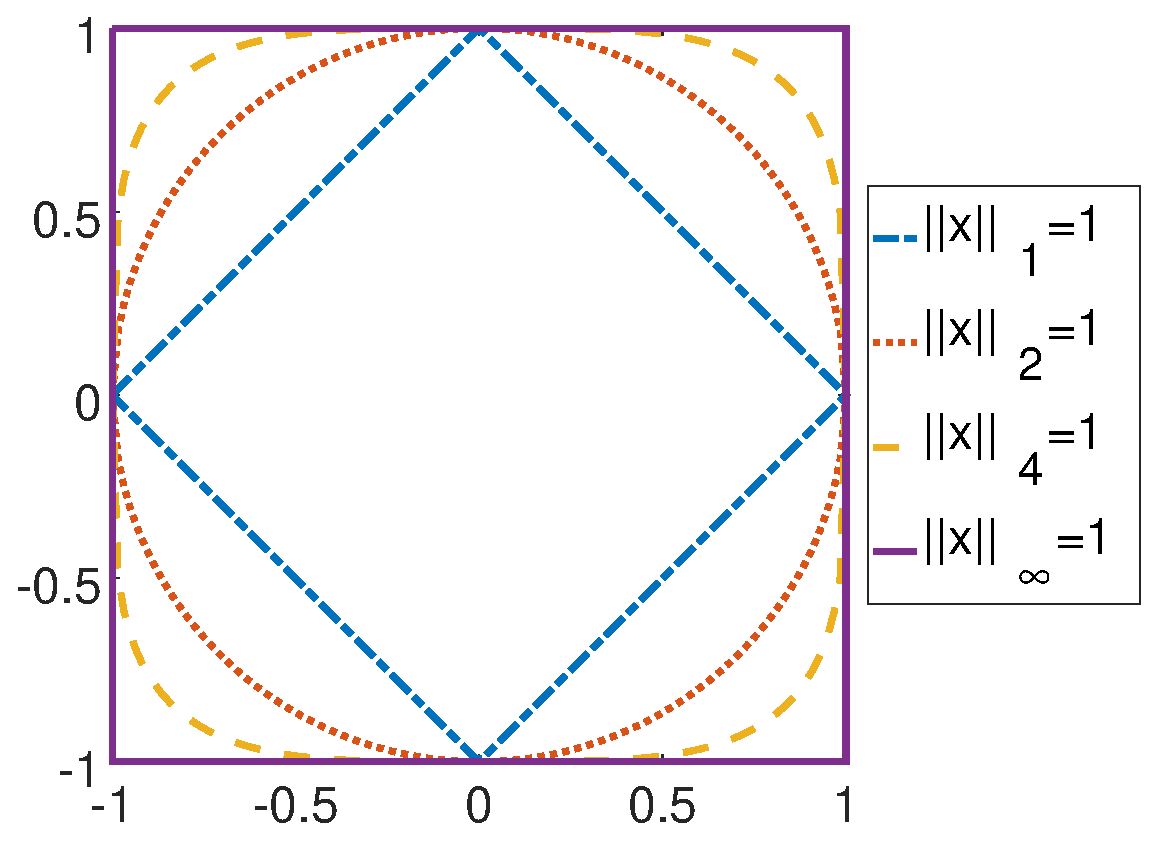
\includegraphics[width=0.45\textwidth]{chapters/notacao/pnormcode.eps}
     \caption{Curva de norma unitária.}
     \label{fig:curvaunit}
     \vspace{-30pt}
\end{wrapfigure}
Dado um vetor $\VECTOR{x} \in \mathbb{C}^{N}$,
é definido a norma $p$ de $\VECTOR{x}$  como $\|\VECTOR{x}\|_p$ \cite[pp. 33]{vetterli2014foundations}, 
\begin{equation}
\|\VECTOR{x}\|_p=\left(\sum_{n=1}^N |x_n|^p\right)^{\frac{1}{p}},
\end{equation}
onde $1 \leq p < \infty$; a norma $p$
também é denotada como norma $L_p$ ou ``$p$-norm'' em inglês.
Assim, dependendo do valor de $p$, entraremos em vários casos ou tipos de norma,
a Fig. \ref{fig:curvaunit} e os seguintes exemplos mostram alguns destes tipos.

\begin{example}[Norma taxicab - $p=1$:] Também chamado norma Manhattan
\begin{equation}
\|\VECTOR{x}\|_1=\sum_{n=1}^N |x_n|.
\end{equation}
\end{example}

\begin{example}[Norma euclidiana - $p=2$:] Também chamada norma euclidiana quadrada, 
esta norma também pode ser representada como $\|\VECTOR{x}\|$ 
de modo que se entende que é a $2$-norm,
\begin{equation}
\|\VECTOR{x}\|_2\equiv \|\VECTOR{x}\| =\sqrt{\sum_{n=1}^N |x_n|^2}.
\end{equation}
Uma representação relativa à norma quadrada euclidiana é
\begin{equation}
\|\VECTOR{x}\|_2^2\equiv \|\VECTOR{x}\|^2=\sum_{n=1}^N |x_n|^2\equiv \VECTOR{x}^{*} \VECTOR{x},
\end{equation}
onde $\VECTOR{x}^{*}\equiv \VECTOR{\bar{x}}^{\transpose}$ 
representa a transposta do conjugado do vetor  $\VECTOR{x}$. 
\end{example}

\begin{example}[Norma com $p=\infty$:]
\begin{equation}
\|\VECTOR{x}\|_{\infty}=\max \left( |x_1|,~|x_2|,~...,~|x_n|,~...,~|x_N|\right)\equiv \max_n \left( |x_n|\right).
\end{equation}
\end{example}


